\documentclass[11pt,a4paper]{article}

% ======================================================================
% Lost in Translation? — final report
% Figures (folder "figures"): design.png, paired_differences.png, similarity_over_time.png
% Code, data and the scripts behind every number: see the repository link on the title page
% ======================================================================

\usepackage[utf8]{inputenc}
\usepackage[T1]{fontenc}
\usepackage{lmodern}
\usepackage[margin=2.5cm]{geometry}
\usepackage{booktabs}
\usepackage{graphicx}
\usepackage{tikz}
\usetikzlibrary{shapes.geometric, arrows.meta, positioning, calc}
\usepackage{xcolor}
\usepackage{microtype}
\usepackage[hidelinks]{hyperref}
\usepackage[round,authoryear]{natbib}
\usepackage{float}
\usepackage{caption}
\captionsetup{font=small}
\setlength{\parskip}{0.3em}

\begin{document}

% ======================================================================
\begin{titlepage}
\centering
{\large Essentials in Text and Speech Processing - Fall Semester 2026\par}
\vspace{2.5cm}
{\LARGE\bfseries Lost in Translation?\par}
\vspace{0.4cm}
{\Large What Machine Translation Changes in Swiss Parliamentary Texts\par}
\vspace{1.5cm}
{\large Klara Kolarova \quad Luisa M\"uller\par}
\vspace{0.4cm}
{\large 20 November 2026\par}
\vspace{1.8cm}
\begin{minipage}{0.86\textwidth}
\small
\noindent\textbf{Abstract.}
Swiss federal law requires official texts in German, French and Italian, and
machine translation (MT) is spreading in federal translation workflows. We ask
what would change if Swiss parliamentary texts were translated by machine
without revision, and whether more recent official translations resemble our model's output more closely, potentially reflecting increased use of MT in translation workflows. We translated 260 motion justifications written by French-speaking members of
parliament into German with an open-weight MT model and compared the output
with the official German translations. The machine output does not uniformly simplify the texts: it uses more common words but longer sentences with deeper dependency structures. It also ignores Swiss writing conventions (\emph{\ss} in 193 of 259
texts, none in the official versions) and frequently loses the legal names of
parliamentary instruments. Over 2000--2025, official translations have become
measurably more similar to the machine output since about 2015, consistent with
increasing MT use, although training-data overlap offers an alternative
explanation. We conclude that MT in this setting requires
professional revision that targets terminology, conventions and sentence
structure.
\end{minipage}
\vfill
{\small Code and data: \url{https://github.com/luisaellamueller/lost-in-translation}\par}
\end{titlepage}

\tableofcontents
\newpage

% ======================================================================
\section{Introduction}
\label{sec:intro}

Switzerland has four national languages, and federal law requires official
texts to be available in German, French and Italian \citep{bk_languages}.
Translation is essential but costly \citep{efd2024}. In 2023, an interpellation
asked about the use of AI tools such as DeepL in federal translation; the
Federal Council answered that essentially no machine-translated official texts
are published without professional review \citep{sommaruga2023}. At the same
time, \citet{canavese2024} show that MT is already part of federal translation
workflows.

Whether review is needed depends on what MT actually changes: not only
\emph{what} is conveyed but \emph{how}, since vocabulary and sentence structure
matter for access to political information \citep{tolochko2019}.

\paragraph{Research questions.}
(RQ1) How do machine translations of Swiss parliamentary texts differ from the
official translations in lexical and grammatical complexity?
(RQ2) Do they respect Swiss writing conventions and parliamentary terminology?
(RQ3) Have official translations become more similar to machine output over time?

\paragraph{Contributions.}
(1) A matched comparison of an open-weight MT model with official Swiss
translations of texts originally written in French; (2) evidence on Swiss
conventions and terminology; (3) an indicator of MT-likeness over 26 years;
(4) a cleaned corpus of 10,573 German--French motion justifications, released
with all translations, measurements and scripts. We do not assess reader
comprehension or the economic value of translation.

% ======================================================================
\section{Background: Machine Translation and Linguistic Complexity}
\label{sec:related}

Machine translation follows the sentence structure of the source text more
closely than human translators do: \citet{luo2024} show that MT is structurally
more conservative than human translation, and post-edited translations show
more interference from the source language than translations from scratch
\citep{toral2019}. Closer preservation of French source structures, including relative clauses, could help explain differences in German sentence length and grammatical structure.

LLM-generated text points the same way: it has longer constituents than human news
text \citep{munozortiz2024}, and ChatGPT essays show greater syntactic complexity,
lower readability \citep{fredrick2025} and more nominalisations \citep{herbold2023}.

Lexically, MT over-uses frequent words and loses rare ones, in statistical and
neural systems alike \citep{vanmassenhove2019lost,vanmassenhove2021machine}, and
post-edited texts are lexically poorer than human translations \citep{toral2019}. This differs from
free text generation, where LLM essays can show greater lexical diversity than
human ones \citep{herbold2023,fredrick2025}; translation constrains the model to
the source and favours its most probable rendering. We therefore
expect easier vocabulary but harder sentences, and measure the two separately,
since complexity is
multidimensional \citep{biber1992}. In Swiss parliamentary debates, complexity
has declined over time, and ChatGPT can simplify the most complex speeches when
asked to \citep{reveilhac2025}; MT is not asked to simplify. If MT makes official
texts syntactically harder, it could reduce their accessibility even when its
vocabulary looks simpler.

\section{Data and Design}
\label{sec:data}

For each selected motion, we compare a machine translation of the French justification with its official German counterpart.

\begin{figure}[tbp]
\centering
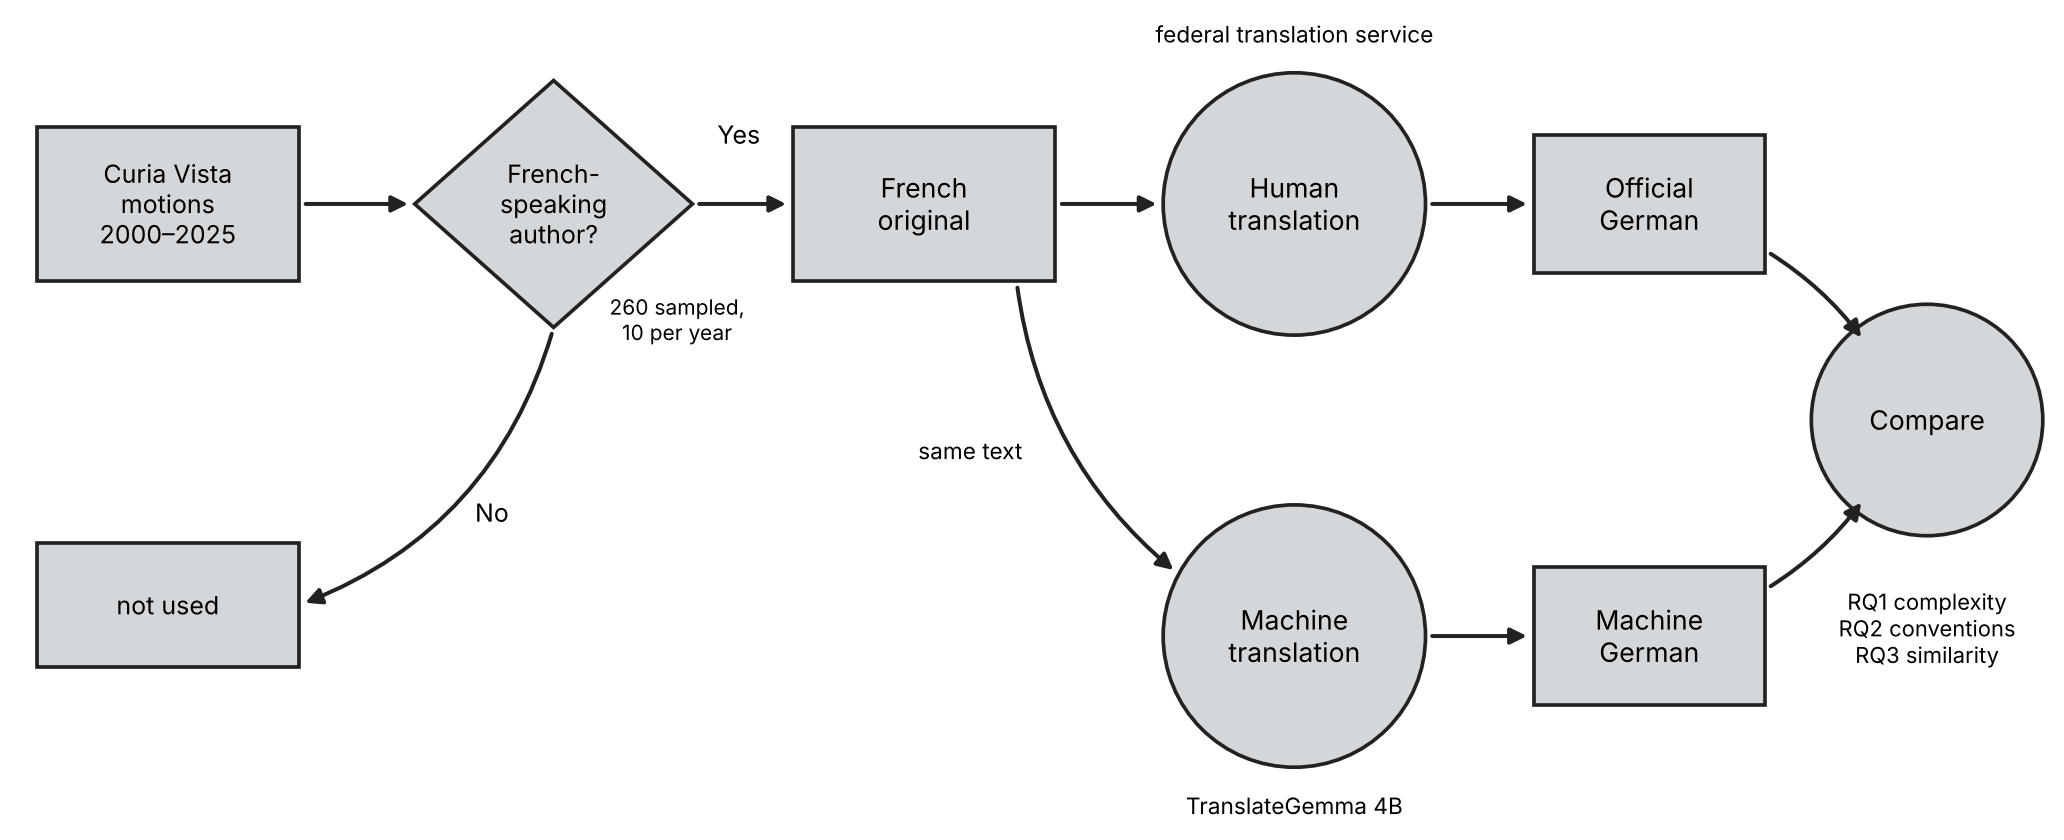
\includegraphics[width=0.78\linewidth]{figures/design.png}
\caption{Experimental design. The same French original is translated once by
the federal translation service (official German) and once by the MT model;
both German versions are then compared.}
\label{fig:design}
\end{figure}

\paragraph{Corpus.} We retrieved all motions submitted 2000--2025 from the Curia
Vista open-data service in German and French and analyse the full justification
(\texttt{ReasonText}). After removing HTML, one duplicated record and 41
entries without an argument, 10,573
German--French pairs remain.

\paragraph{Original language.} Curia Vista does not record the language a motion
was written in. We infer it from the submitting member: the language of a monolingual canton, or for the
bilingual cantons BE, FR, VS and GR the language of the member's biography text,
which matched the canton language for 473 of 475 members from monolingual
cantons where both were available. Committees and parliamentary groups have no single
author language. By this proxy, 2,245 pairs were written by French speakers.

\paragraph{Sample.} We drew ten French-authored pairs per submission year (260),
at random with a fixed seed, excluding 30 documents used to develop the
measures. This restriction reduces the risk of translating a French translation back into its original German, although the author's inferred language is not a completely reliable proxy for the original language of each motion.

\paragraph{Translation.} We translated the French texts with TranslateGemma~4B
\citep{translategemma} (Q4\_K\_M, llama-cpp-python) using its own prompt template,
temperature 0 and seed 42; the model never saw the German reference. One long text reached the output limit and is
reported as a failure, leaving 259 pairs. We chose this model because it is built
for translation and its weights are public: it runs locally with a fixed version,
settings and seed, so every output can be regenerated, and its smaller variants
match much larger general-purpose models \citep{translategemma}. Commercial
systems such as DeepL are updated without versioning, so their outputs cannot be
reproduced later.

\paragraph{Measures.} Both German versions are processed identically with spaCy
\citep{spacy} and wordfreq \citep{wordfreq}. We report seven measures, one or
two per dimension of complexity \citep{biber1992}:
\emph{words per sentence};
\emph{mean sentence-level maximum dependency-tree depth}, measuring the deepest chain of grammatical dependencies in each sentence and averaging across sentences; \emph{subordinate} and \emph{relative clause markers per 100 alphabetic words}
(e.g.\ \emph{dass}, \emph{weil}; \emph{der}, \emph{welche}), a common proxy for
clausal embedding, although marker counts do not always correspond to true
subordination \citep{schleppegrell1992};
\emph{content-word frequency} on the logarithmic Zipf scale (higher = more
common words);
\emph{lexical variety} as the lemma-based moving-average type--token ratio (MATTR, \citealp{covington2010}) over 50-word windows; and the readability index \emph{LIX} \citep{bjornsson1968}, which combines sentence length and the share
of long words (higher = harder). The measures were fixed after a pilot of 30 documents; eleven further measures
are reported in the repository.

\paragraph{Analysis.} For each measure we report the mean paired difference
(machine minus official) with a 95\% interval from 2,000 bootstrap resamples of
document pairs within year. As 60 of 102 authors wrote several texts, we also fit a mixed
model with author random intercepts, Bonferroni-corrected for seven measures. For RQ2 we count Swiss conventions and check whether
the parliamentary terms of the French source reappear in each German version. For
RQ3 we compute the similarity of official and machine German per document with
chrF \citep{popovic2015}, with BLEU \citep{papineni2002} as a robustness check
(sacreBLEU, \citealp{post2018}); this metric was fixed before inspecting results.

\paragraph{Exploratory source comparison.} For all 259 completed translations, we compared sentence counts with the French source using punctuation and line boundaries, with punctuation-only segmentation as a sensitivity check. We parsed French with spaCy \texttt{fr\_core\_news\_sm} (3.8.0) and computed document-level Pearson correlations between source and target mean dependency-tree depth. To account for sentence length, we also correlated residuals after separately regressing depth on mean sentence length in each version. Exploratory 95\% intervals for correlation differences use 2,000 paired bootstrap resamples within year; unlike the primary analysis, they are not adjusted for repeated authors or multiple comparisons.

% ======================================================================
\section{Results}
\label{sec:results}

\subsection{MT shifts complexity from words to sentences (RQ1)}

Figure~\ref{fig:paired} compares the two German versions. The machine output uses
more common content words (+0.12 Zipf, about 1.3 times more frequent; higher in 200 of 259 pairs) and slightly lower lexical variety. The word-frequency difference remains positive when words with zero frequency scores are excluded (+0.072 Zipf; 95\% CI [0.056, 0.088]). Its sentences, however, are longer (+1.1 words), more deeply nested (+0.28 levels) and contain 15\% more
subordinate and 27\% more relative clause markers; the readability index LIX rises by 1.8 points. We found no clear evidence of differences in dependency distance or lexical density. MT therefore does not uniformly simplify the texts: it uses more common vocabulary alongside longer sentences and deeper dependency structures, consistent with the source-structure transfer described for MT \citep{luo2024} and with the greater syntactic complexity reported for AI-generated text \citep{munozortiz2024,fredrick2025}. The directions are the same in 2000--2008, 2009--2016 and 2017--2025, and all seven remain non-zero in the author-adjusted, corrected model.

\begin{figure}[H]
\centering
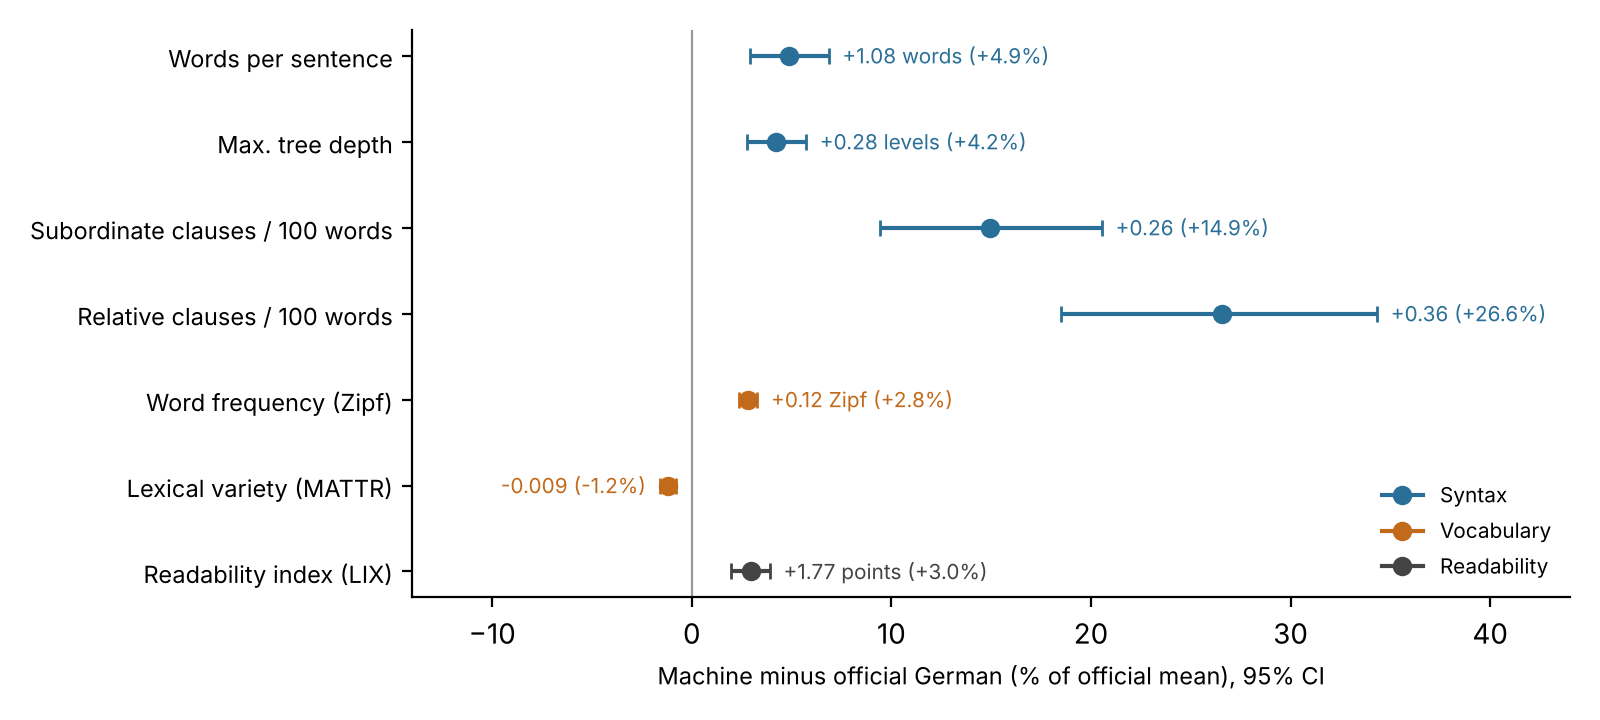
\includegraphics[width=0.92\linewidth]{figures/paired_differences.png}
\caption{Machine minus official German (259 pairs) as a percentage of the
official mean, with 95\% bootstrap intervals; labels give the raw difference.
Zipf is logarithmic: +0.12 means content words are about 1.3 times more
frequent. Higher LIX means harder to read.}
\label{fig:paired}
\end{figure}

\paragraph{Source-structure preservation.} The model matched the French source's sentence count in 166 of 259 texts (64\%), compared with 86 (33\%) for official translations; the pattern persisted with punctuation-only segmentation (164 versus 86). Source and target mean tree depth correlated more strongly for model translations ($r=0.69$) than official translations ($r=0.53$). After adjustment for sentence length, the correlations were 0.43 and 0.26, respectively (difference 0.17; exploratory 95\% CI [0.04, 0.30]). These findings are consistent with closer preservation of source structure, but do not establish matching sentence boundaries or syntactic constructions.

\subsection{MT ignores Swiss conventions and terminology (RQ2)}

Official Swiss German never uses \emph{\ss}, writes thousands as
\emph{10\,000} or \emph{10'000} and uses fixed names for parliamentary
instruments that carry legal meaning: a \emph{Motion} obliges the government to
act, a \emph{Postulat} asks for a report, an \emph{Interpellation} asks
questions. In the 259 pairs, the official translations never use \emph{\ss}; the
machine output does in 193 texts. It writes \emph{10.000} (34 texts, official:
3), never the Swiss forms (official: 32), and German instead of Swiss quotation
marks. Checking every parliamentary term in context (Table~\ref{tab:terms}), the
official translations keep the names of the instruments, whereas the machine
output replaces them with everyday words that name a different procedure: \emph{Interpellation} becomes \emph{Anfrage} in 12 of 15
texts, \emph{Motion} becomes \emph{Antrag} in 18 of 43, and \emph{Postulat}
survives once in four texts. The model also keeps French abbreviations of Swiss
authorities and laws (\emph{AVS} for \emph{AHV}, \emph{LAMal} for \emph{KVG})
in 41 of the 54 texts that contain one; the official translations never do.

\begin{table}[H]
\centering
\small
\setlength{\tabcolsep}{4pt}
\begin{tabular}{llrrrl}
\toprule
French source & Swiss term & Texts & Off. & MT & MT instead (texts) \\
\midrule
\emph{motion} & Motion & 43 & 41 & 22 & \emph{Antrag} (18), other (3) \\
\emph{interpellation} & Interpellation & 15 & 14 & 1 & \emph{Anfrage} (12), lost (2) \\
\emph{postulat} & Postulat & 4 & 4 & 1 & \emph{Petition}, \emph{Punkt}, \emph{Pr\"amisse} \\
\emph{initiative parl.} & Parl.\ Initiative & 2 & 2 & 2 & -- \\
\emph{Conseil f\'ed\'eral} & Bundesrat & 108 & 108 & 95 & \emph{Bundesregierung} (12), other (1) \\
\emph{Conseil des Etats} & St\"anderat & 3 & 3 & 2 & \emph{Rat der St\"ande} (1) \\
\bottomrule
\end{tabular}
\caption{Texts in which the Swiss term named in the French source appears in the
official (Off.) and machine (MT) German. ``Lost'': sentence dropped or mistranslated.}
\label{tab:terms}
\end{table}

\paragraph{Screening of the machine output.} All 259 outputs ended normally. Automatic screening and inspection of flagged cases identified no untranslated French passages or repetition beyond that present in the source; output length is 0.73--1.03 times the French word count (official median 0.91, machine
0.86). Reading the opening (about 100 words) of 20 randomly drawn outputs against the
source, we found ten without problems, five with minor grammatical or stylistic
flaws and five with errors that change content, for example a wrong number
(\emph{145 milliards} $\rightarrow$ \emph{14,5 Milliarden}), a wrong legal term
(\emph{poursuites} $\rightarrow$ \emph{Klagen} instead of \emph{Betreibungen})
and a wrong place name (\emph{Valais} $\rightarrow$ \emph{Waals}).

\subsection{Official translations move towards MT output (RQ3)}

Figure~\ref{fig:similarity} shows how similar the official translations are to
the machine output of the same source. Similarity is flat or slightly falling
until 2010--2014 (chrF 55.9) and then rises steadily to 61.4 in 2023--2025; the
intervals of these two periods do not overlap. The linear trend is +1.6 chrF per
decade (95\% interval +0.8 to +2.5), and BLEU rises from 17 to 24. The turning
point coincides with the spread of neural MT. In line with post-editing research \citep{toral2019}, this is consistent with official
translations increasingly being produced from MT output. It is, however, also
what we would observe if the model had seen recent official translations during training; the two cannot be separated with our data, but texts published after the model's release would help assess whether the pattern persists without direct overlap with its training data.

\begin{figure}[H]
\centering
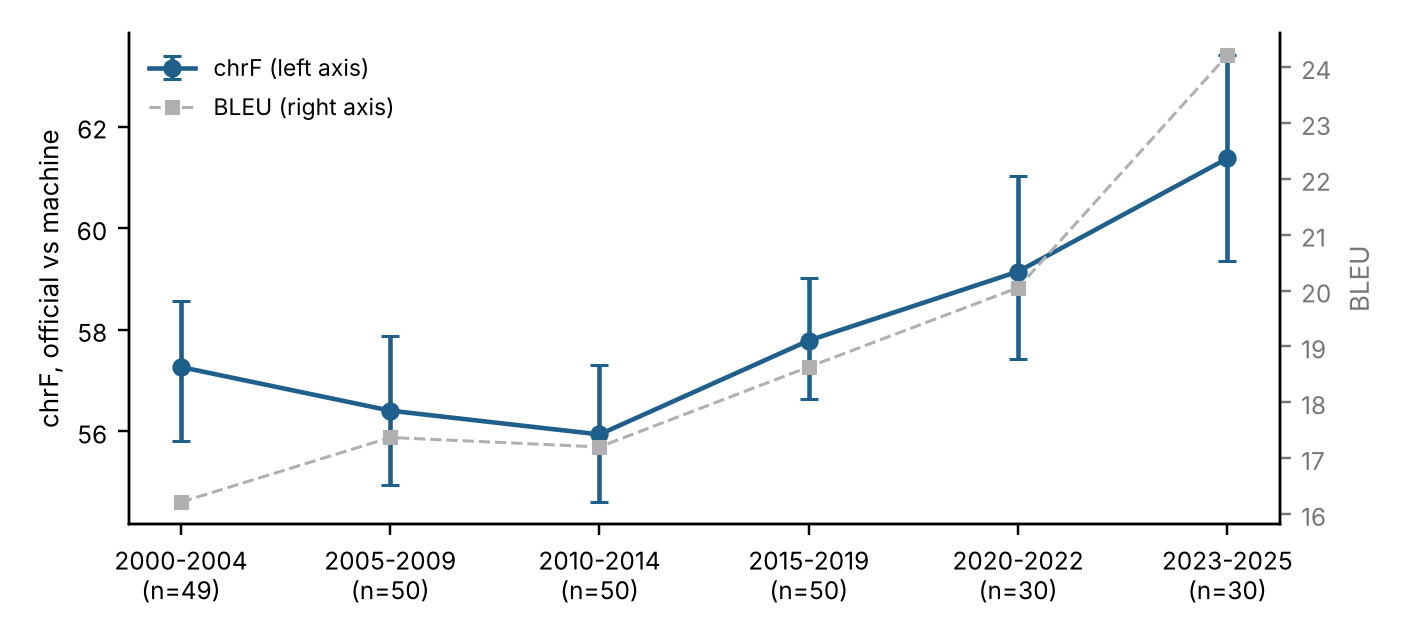
\includegraphics[width=0.62\linewidth]{figures/similarity_over_time.png}
\caption{Similarity between official and machine German translations of the
same French text by period (French-authored sample). chrF with 95\% bootstrap
intervals; BLEU on the right axis.}
\label{fig:similarity}
\end{figure}
Spelling, in contrast, shows no trace of unrevised MT in the official
translations (Table~\ref{tab:ss_dash}). Because Curia Vista stores several special characters faithfully only from
2023 onwards,\footnote{Before 2023 the API returns plain substitutes for guillemets, dashes
and \emph{\oe}: of 8,825 French justifications, 1,381 write \emph{oeuvre}, 2
\emph{\oe uvre} and 5 contain guillemets (2023--2025: 80, 259 and 431 of 1,784).
Whether \emph{\ss} was converted cannot be determined.}
we restrict character-level comparisons to 2023--2025. Our model writes \emph{\ss} in 193 of
259 German translations, but none of the 435 official German translations of
motions written in French (2023--2025) contains it. The 14 official German
texts that do contain \emph{\ss} (e.g.\ \emph{Ma\ss nahmen}, \emph{gem\"a\ss})
were all submitted by individual members who are not French-speaking (12
members; 13 texts by German-speaking members, one by a member from Ticino), so
they were most likely written in German rather than translated. If \emph{\ss}
were spread independently of the original language, the chance that no
translation contained it would be below 1\% (one-sided Fisher's exact test, $p = 0.008$). Dashes, which our
model inserts more often than official translators (37 vs.\ 8 of 259 texts),
rose in 2023--2025 in translated and untranslated texts alike. Overall, the surface errors frequent in our model's output are largely absent from official translations, suggesting professional revision or other quality-control practices.
\begin{table}[H]
\centering
\small
\begin{tabular}{lrrr}
\toprule
 & Texts & with \emph{\ss} & with dash (--) \\
\midrule
Our MT model (German output, all years) & 259 & 193 & 37 \\
Official German translations of motions written in French & 435 & 0 & 91 \\
Official German texts by German- or Italian-speaking members & 1,061 & 14 & 217 \\
\bottomrule
\end{tabular}
\caption{Number of texts containing \emph{\ss} or a dash. Official texts:
2023--2025; motions by committees and parliamentary groups are excluded. }
\label{tab:ss_dash}
\end{table}
% ======================================================================
\section{Discussion}
\label{sec:discussion}

First, unrevised MT changes the complexity profile of parliamentary texts: more common vocabulary accompanies longer sentences and deeper dependency structures. Whether these changes improve or reduce accessibility would require testing with readers. Second, our model frequently departs from Swiss spelling conventions and institutional terminology, whereas the official translations largely preserve them. In official documents, incorrect translations of institutional and legal terms can have consequences for legal interpretation. Third, more recent official translations more closely resemble outputs of our model. If this partly reflects increased use of MT in translation workflows, our findings highlight features that translators should pay particular attention to when revising machine-generated drafts. The findings support the Federal Council's position that MT output needs professional review, and show where it should focus. Conventions and terminology could be addressed in part through automated checks, such as converting \emph{\ss} to \emph{ss} and checking translations against a glossary of parliamentary terms; human review remains important for meaning and sentence structure.

\paragraph{Limitations.} We evaluate one open-weight model; the administration more likely uses commercial systems. The original language is inferred from the submitting member, a proxy. Our measures are parser-based estimates, not reader tests, and translation quality is assessed only through the terminology check and a screening. French and German parsers use different annotation schemes, so the exploratory source comparison measures document-level covariation rather than directly equivalent dependency trees. Spot-checking also revealed a relative pronoun incorrectly tagged as an article, illustrating how tagging errors can affect clause-marker counts. The similarity trend may partly reflect training-data overlap, and topics vary over time.

% ======================================================================
\section{Conclusion}

Our model's unrevised translations show systematic differences from the official German versions: more common vocabulary alongside longer sentences and deeper dependency structures, departures from Swiss writing conventions, and errors in institutional terminology. The terminology errors and departures from Swiss conventions identified in our model's output highlight the importance of targeted revision before publication. Future work should add commercial MT systems and reader studies.

% ======================================================================

\begin{thebibliography}{99}
\setlength{\itemsep}{1pt}
\small

\bibitem[Biber(1992)]{biber1992}
D.~Biber. 1992. On the complexity of discourse complexity: A multidimensional
analysis. \emph{Discourse Processes}, 15(2):133--163.
\href{https://doi.org/10.1080/01638539209544806}{doi:10.1080/01638539209544806}.

\bibitem[Bj{\"o}rnsson(1968)]{bjornsson1968}
C.~H. Bj{\"o}rnsson. 1968. \emph{L{\"a}sbarhet}. Liber, Stockholm.

\bibitem[Canavese and Cadwell(2024)]{canavese2024}
P.~Canavese and P.~Cadwell. 2024. Translators' perspectives on machine
translation uses and impacts in the Swiss Confederation. In \emph{Proceedings of
EAMT 2024}, pages 347--359. \href{https://aclanthology.org/2024.eamt-1.30/}{aclanthology.org/2024.eamt-1.30/}.

\bibitem[Covington and McFall(2010)]{covington2010}
M.~A. Covington and J.~D. McFall. 2010. Cutting the Gordian knot: The
moving-average type--token ratio (MATTR). \emph{Journal of Quantitative
Linguistics}, 17(2):94--100.

\bibitem[EFD(2024)]{efd2024}
Expertengruppe Aufgaben- und Subventions\"uberpr\"ufung. 2024.
\emph{Aufgaben- und Subventions\"uberpr\"ufung 2024: Bericht der Expertengruppe
zuhanden des Bundesrates}. Eidgen\"ossisches Finanzdepartement.
\href{https://www.newsd.admin.ch/newsd/message/attachments/89485.pdf}{www.newsd.admin.ch/newsd/message/attachments/89485.pdf}.

\bibitem[Fredrick and Craven(2025)]{fredrick2025}
D.~R. Fredrick and L.~Craven. 2025. Lexical diversity, syntactic complexity, and
readability: a corpus-based analysis of ChatGPT and L2 student essays.
\emph{Frontiers in Education}, 10:1616935. \href{https://doi.org/10.3389/feduc.2025.1616935}{doi:10.3389/feduc.2025.1616935}.

\bibitem[Herbold et~al.(2023)]{herbold2023}
S.~Herbold, A.~Hautli-Janisz, U.~Heuer, Z.~Kikteva and A.~Trautsch. 2023. AI,
write an essay for me: A large-scale comparison of human-written versus
ChatGPT-generated essays. \emph{Scientific Reports}, 13:18617.
\href{https://doi.org/10.1038/s41598-023-45644-9}{doi:10.1038/s41598-023-45644-9}.

\bibitem[Honnibal et~al.(2020)]{spacy}
M.~Honnibal, I.~Montani, S.~Van~Landeghem and A.~Boyd. 2020. spaCy:
Industrial-strength natural language processing in Python.
\href{https://doi.org/10.5281/zenodo.1212303}{doi:10.5281/zenodo.1212303}.

\bibitem[Luo et~al.(2024)]{luo2024}
J.~Luo, C.~Cherry and G.~Foster. 2024. To diverge or not to diverge: A
morphosyntactic perspective on machine translation vs human translation.
\emph{Transactions of the ACL}, 12:355--371. \href{https://aclanthology.org/2024.tacl-1.20/}{aclanthology.org/2024.tacl-1.20/}.

\bibitem[Mu{\~n}oz-Ortiz et~al.(2024)]{munozortiz2024}
A.~Mu{\~n}oz-Ortiz, C.~G{\'o}mez-Rodr{\'i}guez and D.~Vilares. 2024. Contrasting
linguistic patterns in human and LLM-generated news text. \emph{Artificial
Intelligence Review}, 57(10). \href{https://doi.org/10.1007/s10462-024-10903-2}{doi:10.1007/s10462-024-10903-2}.

\bibitem[Papineni et~al.(2002)]{papineni2002}
K.~Papineni, S.~Roukos, T.~Ward and W.-J. Zhu. 2002. BLEU: a method for automatic
evaluation of machine translation. In \emph{Proceedings of ACL 2002}, pages
311--318. \href{https://aclanthology.org/P02-1040/}{aclanthology.org/P02-1040/}.

\bibitem[Popovi{\'c}(2015)]{popovic2015}
M.~Popovi{\'c}. 2015. chrF: character n-gram F-score for automatic MT evaluation.
In \emph{Proceedings of the Tenth Workshop on Statistical Machine Translation},
pages 392--395. \href{https://aclanthology.org/W15-3049/}{aclanthology.org/W15-3049/}.

\bibitem[Post(2018)]{post2018}
M.~Post. 2018. A call for clarity in reporting BLEU scores. In \emph{Proceedings
of the Third Conference on Machine Translation}, pages 186--191. \href{https://aclanthology.org/W18-6319/}{aclanthology.org/W18-6319/}.

\bibitem[Reveilhac and Schneider(2025)]{reveilhac2025}
M.~Reveilhac and G.~Schneider. 2025. Measuring language complexity about
European politics in Swiss parliamentary debates. In \emph{Mathematical
Modelling in Linguistics and Text Analysis}, Current Issues in Linguistic Theory
370, pages 191--206. John Benjamins. \href{https://doi.org/10.1075/cilt.370.16rev}{doi:10.1075/cilt.370.16rev}.

\bibitem[Schleppegrell(1992)]{schleppegrell1992}
M.~J. Schleppegrell. 1992. Subordination and linguistic complexity.
\emph{Discourse Processes}, 15(1):117--131. \href{https://benjamins.com/online/ebop/publications/23138}{benjamins.com/online/ebop/publications/23138}.

\bibitem[Sommaruga(2023)]{sommaruga2023}
C.~Sommaruga. 2023. \"Ubersetzung in der Bundesverwaltung. Gef\"ahrdung eines Berufs
durch Lohndumping und Einsatz k\"unstlicher Intelligenz. Interpellation 23.4489,
Swiss Parliament. \href{https://www.parlament.ch/de/ratsbetrieb/suche-curia-vista/geschaeft?AffairId=20234489}{parlament.ch, Curia Vista 23.4489}.

\bibitem[Speer(2023)]{wordfreq}
R.~Speer. 2023. wordfreq, version 3.1.1. Python package.
\href{https://github.com/rspeer/wordfreq}{github.com/rspeer/wordfreq}.

\bibitem[Swiss Federal Chancellery(2026)]{bk_languages}
Swiss Federal Chancellery. Languages. \href{https://www.bk.admin.ch/en/languages}{www.bk.admin.ch/en/languages}.
Accessed 13 September 2026.

\bibitem[Tolochko et~al.(2019)]{tolochko2019}
P.~Tolochko, H.~Song and H.~Boomgaarden. 2019. ``That looks hard!'': Effects of
objective and perceived textual complexity on factual and structural political
knowledge. \emph{Political Communication}, 36(4):609--628.
\href{https://doi.org/10.1080/10584609.2019.1631919}{doi:10.1080/10584609.2019.1631919}.

\bibitem[Toral(2019)]{toral2019}
A.~Toral. 2019. Post-editese: an exacerbated translationese. In
\emph{Proceedings of Machine Translation Summit XVII}, pages 273--281.
\href{https://aclanthology.org/W19-6627/}{aclanthology.org/W19-6627/}.

\bibitem[Google Translate Research Team(2026)]{translategemma}
Google Translate Research Team. 2026. TranslateGemma technical report.
\href{https://arxiv.org/abs/2601.09012}{arXiv:2601.09012}.

\bibitem[Vanmassenhove et~al.(2019)]{vanmassenhove2019lost}
E.~Vanmassenhove, D.~Shterionov and A.~Way. 2019. Lost in translation: Loss and
decay of linguistic richness in machine translation. In \emph{Proceedings of
Machine Translation Summit XVII}, pages 222--232. \href{https://aclanthology.org/W19-6622/}{aclanthology.org/W19-6622/}.

\bibitem[Vanmassenhove et~al.(2021)]{vanmassenhove2021machine}
E.~Vanmassenhove, D.~Shterionov and M.~Gwilliam. 2021. Machine translationese:
Effects of algorithmic bias on linguistic complexity in machine translation. In
\emph{Proceedings of EACL 2021}, pages 2203--2213.
\href{https://aclanthology.org/2021.eacl-main.188/}{aclanthology.org/2021.eacl-main.188/}.

\end{thebibliography}

\end{document},
